\documentclass[12pt]{article}
\usepackage[utf8]{inputenc}
\usepackage{amsmath, amssymb, mathtools}
\usepackage{geometry}
\geometry{a4paper, margin=1in}
\usepackage{enumitem}
\usepackage{hyperref}
\usepackage{mathrsfs}
\usepackage{amsfonts}
\usepackage{bbm}
\usepackage{xcolor}
\usepackage{tikz}
\usetikzlibrary{shapes.geometric, arrows.meta, positioning}
\usepackage{tikz-cd}
\usepackage{listings}
\lstset{language=Haskell, basicstyle=\ttfamily\small, breaklines=true, frame=single}
\usepackage{lmodern}

\title{Semantic Infrastructure: Entropy-Respecting Computation in a Modular Universe}
\author{}
\date{August 2025}

\begin{document}

\maketitle

\begin{abstract}
This monograph proposes a foundational framework for semantic modular computation grounded in the principles of the Relativistic Scalar Vector Plenum (RSVP) theory, category theory, and sheaf-theoretic structure. Moving beyond file-based version control systems like GitHub, we define a symmetric monoidal $\infty$-category of semantic modules, equipped with a homotopy-colimit-based merge operator that resolves computational and conceptual divergences through higher coherence.

Each semantic module is modeled as an entropy-respecting construct, encoding functions, theories, and transformations as type-safe, sheaf-gluable, and obstruction-aware structures. We introduce a formal merge operator derived from obstruction theory, cotangent complexes, and mapping stacks, capable of resolving multi-way semantic merges across divergent forks. The system integrates deeply with RSVP field logic, treating code and concept as flows within a plenum of semantic energy.

We propose implementations in Haskell using dependent types, lens-based traversals, and type-indexed graphs, along with potential extensions to blockchain-based identity tracking, Docker-integrated module deployment, and a latent space knowledge graph for semantic traversal.

This monograph provides the formal infrastructure for a new kind of open, modular, intelligent computation—where meaning composes, entropy flows, and semantic structure becomes executable.
\end{abstract}

\section*{Introduction}
\subsection*{Motivation}
The modern paradigm of software development, exemplified by platforms like GitHub, suffers from deep limitations:
\begin{itemize}
    \item Namespaces are symbolic and fragile
    \item Version control is syntactic, not semantic
    \item Merges are line-based diffs, not concept-aware integrations
    \item Forks create fragmentation, not divergence-preserving structure
\end{itemize}
These limitations stem from a fundamental misalignment between how we encode meaning and how we operationalize computation. This monograph proposes a radical alternative: a semantic, compositional, entropy-respecting infrastructure for computation, theory, and collaboration.

\subsection*{Philosophical Foundations}
Drawing from the RSVP theory, we treat computation as structured flows of entropy and coherence through scalar, vector, and entropy fields. Each module is a local condensation of meaning, and its integration into larger systems must reflect not just syntax, but thermodynamic, categorical, and topological consistency.

We borrow tools from:
\begin{itemize}
    \item Category theory: for structure, morphisms, and functoriality
    \item Sheaf theory: for local-to-global consistency and gluing
    \item Obstruction theory: for precise conditions on mergeability
    \item Homotopy theory: for higher-order coherence between divergent views
    \item Haskell and type theory: for practical implementation
\end{itemize}
This monograph develops a full formal system to replace platform-centric collaboration with semantic infrastructure rooted in mathematics, physics, and coherent modularity.

\tableofcontents

\part{Foundations}

\section{From Source Control to Semantic Computation}
\subsection{The GitHub Illusion: Permissions Masquerading as Namespace}
The current global infrastructure for collaborative coding—centered around platforms like GitHub, GitLab, and Bitbucket—presents itself as a coherent namespace for projects, contributors, and computational modules. This appearance is deceptive. Beneath its clean user interface and social coding veneer, GitHub operates as a permissioned layer over traditional file systems and symbolic version control. Its structure is not ontological but operational: it organizes who can read, write, and execute, not what things are or how they relate.

GitHub repositories are little more than glorified \texttt{\~/user/project} directories with cosmetic metadata. Branches simulate multiplicity, but are essentially temporal forks of file state. The underlying Git system, while ingenious in its content-based commit hashing and tree structure, still anchors meaning to syntax: merge conflicts are lines in a file, not semantic contradictions. There is no awareness of function, type, theory, or ontology. A function called \texttt{transform()} in two branches may represent wildly different concepts, yet GitHub cannot tell. Names collide. Meaning does not.

Worse still, forking creates epistemic fragmentation. Semantic divergence—two people exploring conceptually related but non-equivalent evolutions of a model—becomes a structural break, rather than a traceable, composable lineage. The illusion of version control is that it preserves change, when in fact it buries intent beneath syntax.

\begin{figure}[h]
    \centering
    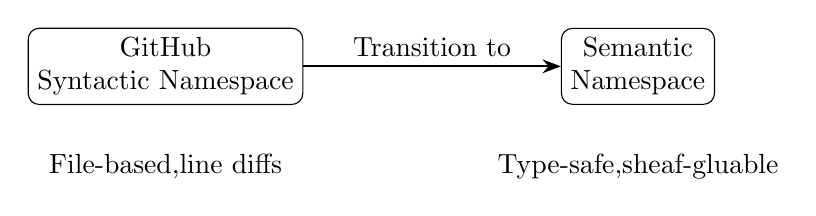
\begin{tikzpicture}[
        box/.style={rectangle, draw, rounded corners, minimum height=2em, minimum width=4em, align=center},
        arrow/.style={-Stealth, thick}
    ]
        \node[box] (git) at (0,0) {GitHub\\Syntactic Namespace};
        \node[box] (semantic) at (6,0) {Semantic\\Namespace};
        \draw[arrow] (git) -- (semantic) node[midway, above] {Transition to};
        \node[below=0.5cm of git] {File-based,\\line diffs};
        \node[below=0.5cm of semantic] {Type-safe,\\sheaf-gluable};
    \end{tikzpicture}
    \caption{Comparison of GitHub's syntactic namespace and the proposed semantic namespace.}
\end{figure}

\subsection{Beyond Line Diffs: Why Semantic Meaning Doesn’t Compose in Git}
The heart of the problem is that Git and GitHub were not designed to handle semantic modules. They were built to track files and textual edits, not functions, proofs, type transformations, or field-theoretic roles. As a result, even modestly complex systems of co-evolving components become brittle, merge-prone, and semantically opaque.

Consider three contributors modifying different aspects of a codebase: one improves a mathematical model, another optimizes the data pipeline, and a third refactors type declarations for clarity. In Git, these become three sets of file-level diffs, potentially colliding in lines or structure. There is no global view of which semantic modules were affected, what dependencies were touched, or how their conceptual alignment changed.

This is not merely a usability issue. It is a representational error. The assumption that text = meaning is false. It fails especially for scientific computing, AI, theory-building, and systems where correctness is determined by more than syntactic compatibility.

Merges in Git fail not because humans can’t reason about them, but because Git has no internal theory of what is being merged.

\subsection{Toward Modular Entropy: Computation as Structured Coherence}
To move beyond this collapse of meaning, we propose a new approach: semantic modular computation. This approach views each computational module not as a file or blob of text, but as a structured field of coherent roles, transformations, and entropic flows. It takes seriously the idea that code, data, and theory are not merely stored, but expressed.

Each module in this framework is treated as a condensate of meaning: a packet of structured entropy, bounded by its dependencies, roles, and transformations. These modules live not in a file system, but in a semantic space indexed by type, function, and ontological role. They are composed not by appending lines or concatenating diffs, but by merging structured flows through higher categorical constructions.

This shift requires a fundamentally different substrate. Instead of Git branches, we need sheaf-theoretic contexts. Instead of line diffs, we need obstruction classes and derived stacks. Instead of symbolic names like \texttt{main} and \texttt{dev}, we need hash-addressed entropy modules with traceable morphisms between semantic states.

Semantic computation is not just a change in tooling; it is a change in worldview. It treats computation as a thermodynamic, categorical, and epistemic process. In the chapters that follow, we will construct the infrastructure needed to make this real: symmetric monoidal categories of semantic modules, merge operators derived from homotopy colimits, and a practical encoding of these ideas in type-safe languages like Haskell.

But we begin here, with a simple insight: GitHub is not a namespace. It is a container. And what we need is not more containers, but a language for meaning that composes.

\section{RSVP Theory and Modular Fields}
\subsection{Scalar ($\Phi$), Vector ($\vec{v}$), and Entropy ($S$) Fields}
The Relativistic Scalar Vector Plenum (RSVP) theory models computation as dynamic interactions within a spacetime manifold $M = \mathbb{R} \times \mathbb{R}^2$ equipped with a Minkowski metric $\eta_{\mu\nu}$. We define three fields:
\begin{itemize}
    \item Scalar field $\Phi: M \to \mathbb{R}$, representing semantic coherence.
    \item Vector field $\vec{v}: M \to T M$, encoding inference flows.
    \item Entropy field $S: M \to \mathbb{R}_{\geq 0}$, capturing uncertainty and divergence.
\end{itemize}
These fields evolve according to stochastic partial differential equations (SPDEs):
\[
d\Phi = \left(D \Delta \Phi - \vec{v} \cdot \nabla \Phi + \lambda S\right) dt + \sigma_\Phi dW_t,
\]
\[
d\vec{v} = \left(-\nabla S + \gamma \Phi \vec{v}\right) dt + \sigma_v dW_t,
\]
\[
dS = \left(\delta \nabla \cdot \vec{v} - \eta S^2\right) dt + \sigma_S dW_t,
\]
where $D, \lambda, \gamma, \delta, \eta$ are parameters, $\Delta$ is the Laplacian, and $W_t$ is a Wiener process. These equations ensure entropy-respecting dynamics, with $\Phi$ stabilizing coherence, $\vec{v}$ directing inference, and $S$ managing uncertainty.

\subsection{Modules as Condensates of Coherent Entropy}
A semantic module is a tuple $M = (F, \Sigma, D, \alpha)$, where:
\begin{itemize}
    \item $F$: Set of function hashes (e.g., SHA-256 of code).
    \item $\Sigma$: Type annotations (dependent types).
    \item $D$: Dependency graph (directed acyclic graph of imports).
    \item $\alpha: \Sigma \to (\Phi, \vec{v}, S)$, mapping types to RSVP fields.
\end{itemize}
Modules are local sections of a sheaf over an open set $U \subseteq M$, ensuring gluable, coherent structures. The entropy field $S$ quantifies the module’s divergence, enabling entropy-respecting composition.

\subsection{Code as Structured Entropic Flow}
Code is modeled as transformations within the RSVP plenum. A function $f \in F$ induces a morphism $f: M \to M'$ in the category of modules, preserving field dynamics. This perspective treats code execution as flows of coherence and entropy, with simulations provided in the Python script \texttt{rsvp\_simulation.py}.

\section{Category-Theoretic Infrastructure}
\subsection{Semantic Modules as Objects in a Fibred Category}
Semantic modules form objects in a symmetric monoidal $\infty$-category $\mathcal{C}$, fibred over a base category of types. An object $M = (F, \Sigma, D, \alpha)$ is equipped with morphisms $f = (f_F, f_\Sigma, f_D, f_\alpha)$ preserving structure.

\subsection{Morphisms, Functors, and Contextual Roles}
Morphisms in $\mathcal{C}$ are type-safe transformations, with functors mapping modules to semantic spaces. Contextual roles are encoded via groupoid structures, allowing reparameterization of modules across contexts.

\subsection{Groupoids for Forks, Lineage, and Reparameterization}
Forks are modeled as groupoids, with objects representing module states and morphisms capturing lineage. Reparameterization ensures semantic consistency across divergent forks.

\part{Sheaves, Stacks, and Semantic Merges}

\section{Sheaf-Theoretic Modular Gluing}
\subsection{Sites and Semantic Covers}
A site on $M$ defines a Grothendieck topology, with open sets $U_i \subseteq M$ forming a semantic cover. Modules are sheaves $\mathcal{F}: \mathcal{O}(M) \to \mathcal{C}$, ensuring local-to-global consistency.

\subsection{Local Sections, Overlap Agreement, and Global Merge}
Local sections $\mathcal{F}(U_i)$ agree on overlaps $U_i \cap U_j$, enabling gluing into a global module. This process is formalized via sheaf cohomology.

\subsection{Sheaves of Semantic Meaning across Theoretical Domains}
Sheaves encode theories (e.g., RSVP, SIT) as sections, allowing cross-domain composition.

\section{Stacks, Derived Categories, and Obstruction}
\subsection{Stacks of Modules: Higher Structures for Forking and Gluing}
Stacks over $\mathcal{C}$ handle higher-order forks, modeled as 2-categories with descent data.

\subsection{Cotangent Complexes and Semantic Deformation Spaces}
The cotangent complex $L_M$ measures deformations in semantic space, detecting merge obstructions.

\subsection{Ext$^n$ Obstructions to Mergeability}
Obstructions are classified via $\text{Ext}^n(L_M, \mathcal{O})$, determining merge feasibility.

\section{Semantic Merge Operator}
\subsection{Formal Definition of $\mu: M_1 \times M_2 \dashrightarrow M$}
The merge operator $\mu: M_1 \times M_2 \dashrightarrow M$ is a partial functor, defined as a pushout in $\mathcal{C}$:
\[
\begin{tikzcd}
M_1 \cap M_2 \arrow[r] \arrow[d] & M_1 \arrow[d] \\
M_2 \arrow[r] & M
\end{tikzcd}
\]
where $M_1 \cap M_2$ is the shared semantic context.

\subsection{Failure Modes and Obstruction Interpretation}
Merge failures occur when $\text{Ext}^1 \neq 0$, interpreted via obstruction theory.

\subsection{RSVP Interpretation of Merge: Entropy Field Alignment}
Merges align RSVP fields, minimizing entropy divergence $S$.

\begin{figure}[h]
    \centering
    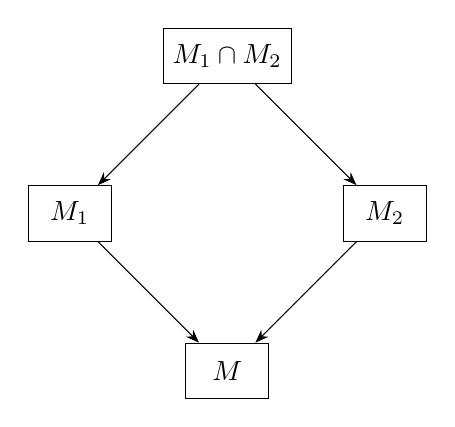
\begin{tikzpicture}[
        box/.style={rectangle, draw, minimum height=2em, minimum width=3em},
        arrow/.style={-Stealth}
    ]
        \node[box] (M12) at (0,2) {$M_1 \cap M_2$};
        \node[box] (M1) at (-2,0) {$M_1$};
        \node[box] (M2) at (2,0) {$M_2$};
        \node[box] (M) at (0,-2) {$M$};
        \draw[arrow] (M12) -- (M1);
        \draw[arrow] (M12) -- (M2);
        \draw[arrow] (M1) -- (M);
        \draw[arrow] (M2) -- (M);
    \end{tikzpicture}
    \caption{Pushout diagram for the semantic merge operator $\mu$.}
\end{figure}

\part{Homotopy, Coherence, and Composition}

\section{Multi-Way Merge via Homotopy Colimit}
\subsection{Merge as Colimit in Diagram of Modules}
Multi-way merges are homotopy colimits $\mathrm{hocolim}_\mathcal{I} D$ over a diagram $D: \mathcal{I} \to \mathcal{C}$ of modules.

\subsection{Higher-Order Forks and Gluing Diagrams}
Higher-order forks are modeled as simplicial objects, with gluing via descent.

\subsection{Extending to $\mathrm{hocolim}_\mathcal{I} D$}
The homotopy colimit extends to infinite forks, ensuring coherence.

\section{Symmetric Monoidal Structure}
\subsection{Defining $\otimes$: Parallel Composition of Modules}
The monoidal product $\otimes: \mathcal{C} \times \mathcal{C} \to \mathcal{C}$ composes modules in parallel:
\[
M_1 \otimes M_2 = (F_1 \cup F_2, \Sigma_1 \times \Sigma_2, D_1 \sqcup D_2, \alpha_1 + \alpha_2).
\]

\subsection{Unit Object and Identity Module}
The unit object is the empty module $I = (\emptyset, \emptyset, \emptyset, 0)$.

\subsection{Merge as Lax Symmetric Monoidal Functor}
The merge operator $\mu$ is lax monoidal, preserving $\otimes$.

\begin{figure}[h]
    \centering
    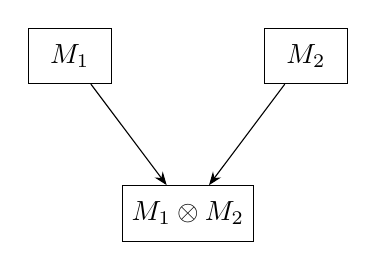
\begin{tikzpicture}[
        box/.style={rectangle, draw, minimum height=2em, minimum width=3em},
        arrow/.style={-Stealth}
    ]
        \node[box] (M1) at (0,0) {$M_1$};
        \node[box] (M2) at (3,0) {$M_2$};
        \node[box] (M12) at (1.5,-2) {$M_1 \otimes M_2$};
        \draw[arrow] (M1) -- (M12);
        \draw[arrow] (M2) -- (M12);
    \end{tikzpicture}
    \caption{Monoidal product of semantic modules.}
\end{figure}

\section{RSVP Entropy Topology and Tiling}
\subsection{Tensor Fields of Entropy Modules}
Modules induce tensor fields on $M$, with entropy $S$ defining a topology.

\subsection{Topological Defects as Merge Obstructions}
Defects in the entropy field correspond to merge failures.

\subsection{Field-Theoretic Interpretation of Semantic Diagrams}
Diagrams are interpreted as field flows, visualized in Appendix F.

\begin{figure}[h]
    \centering
    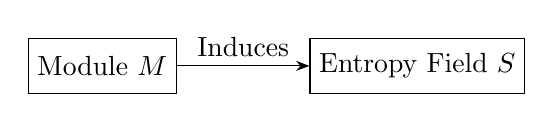
\begin{tikzpicture}[
        box/.style={rectangle, draw, minimum height=2em, minimum width=3em},
        arrow/.style={-Stealth}
    ]
        \node[box] (M) at (0,0) {Module $M$};
        \node[box] (S) at (4,0) {Entropy Field $S$};
        \draw[arrow] (M) -- (S) node[midway, above] {Induces};
    \end{tikzpicture}
    \caption{Module inducing entropy field topology.}
\end{figure}

\part{Implementation and Infrastructure}

\section{Haskell Encoding of Semantic Modules}
\subsection{Type-Level Semantics and Function Hashes}
Semantic modules are encoded in Haskell (see Appendix E), with functions hashed via SHA-256.

\subsection{Lens-Based Traversals and Fork Morphisms}
Lenses enable type-safe traversals of module dependencies.

\subsection{Graphs of Modules as Type-Safe Quivers}
Dependency graphs are quivers in $\mathcal{C}$, implemented via GADTs.

\section{Latent Space Embedding and Knowledge Graphs}
\subsection{Functors $\Phi: \mathcal{M} \to \mathbb{R}^n$ and Similarity Metrics}
Modules are embedded into $\mathbb{R}^n$ via functors, with Gromov-Wasserstein metrics for similarity.

\subsection{Derived Concept Graphs and Gromov-Wasserstein Metrics}
Concept graphs are derived from module dependencies, visualized as knowledge graphs.

\subsection{Visualizing and Traversing Entropy-Structured Semantic Space}
Simulations in \texttt{rsvp\_simulation.py} visualize field embeddings.

\begin{figure}[h]
    \centering
    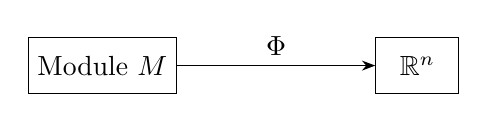
\begin{tikzpicture}[
        box/.style={rectangle, draw, minimum height=2em, minimum width=3em},
        arrow/.style={-Stealth}
    ]
        \node[box] (M) at (0,0) {Module $M$};
        \node[box] (R) at (4,0) {$\mathbb{R}^n$};
        \draw[arrow] (M) -- (R) node[midway, above] {$\Phi$};
    \end{tikzpicture}
    \caption{Latent space embedding of a module.}
\end{figure}

\section{Deployment Architecture}
\subsection{Blockchain-Based Identity and Semantic Versioning}
Module identities are tracked via blockchain, ensuring semantic versioning.

\subsection{Docker/Kubernetes-Backed Module Distribution}
Modules are containerized for scalable deployment.

\subsection{Replacing GitHub and Hugging Face with Semantic Substrates}
A new substrate integrates RSVP and category-theoretic principles.

\begin{figure}[h]
    \centering
    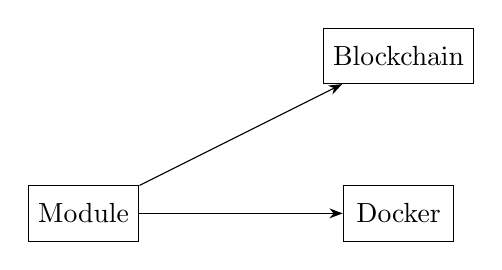
\begin{tikzpicture}[
        box/.style={rectangle, draw, minimum height=2em, minimum width=4em},
        arrow/.style={-Stealth}
    ]
        \node[box] (M) at (0,0) {Module};
        \node[box] (D) at (4,0) {Docker};
        \node[box] (B) at (4,2) {Blockchain};
        \draw[arrow] (M) -- (D);
        \draw[arrow] (M) -- (B);
    \end{tikzpicture}
    \caption{Deployment architecture.}
\end{figure}

\part{Philosophical and Epistemic Implications}

\section{What It Means to Compose Meaning}
\subsection{Beyond Files: Ontological Boundaries in Computation}
Computation is redefined as ontological composition, not file manipulation.

\subsection{Modular Cognition and Conscious Infrastructure}
Modules reflect cognitive structures, enabling conscious computation.

\subsection{Code as Ontological Architecture}
Code becomes an architectural framework for meaning.

\section{Plural Ontologies and Polysemantic Merge}
\subsection{Sheaves Across Worlds: RSVP, SIT, CoM, RAT, etc.}
Sheaves unify ontologies (RSVP, SIT) across semantic domains.

\subsection{Merge as Metaphysical Reconciliation}
Merges reconcile divergent worldviews.

\subsection{Toward a Universal Computable Multiverse}
The framework supports a multiverse of computable meanings.

\begin{figure}[h]
    \centering
    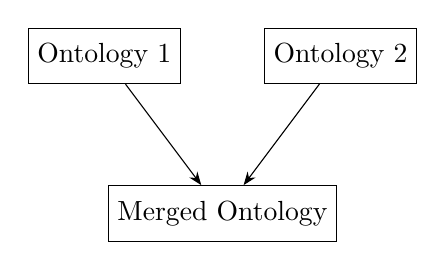
\begin{tikzpicture}[
        box/.style={rectangle, draw, minimum height=2em, minimum width=3em},
        arrow/.style={-Stealth}
    ]
        \node[box] (M1) at (0,0) {Ontology 1};
        \node[box] (M2) at (3,0) {Ontology 2};
        \node[box] (M) at (1.5,-2) {Merged Ontology};
        \draw[arrow] (M1) -- (M);
        \draw[arrow] (M2) -- (M);
    \end{tikzpicture}
    \caption{Polysemantic merge across ontologies.}
\end{figure}

\appendix

\section{Categorical Infrastructure of Modules}
Semantic modules are objects in $\mathcal{C}$, with morphisms preserving RSVP fields. The category is fibred over types, with functors to semantic spaces.

\section{Sheaf-Theoretic Merge Conditions}
Merges satisfy sheaf gluing conditions, with $\mathcal{F}(U_1 \cup U_2) \cong \mathcal{F}(U_1) \times_{\mathcal{F}(U_1 \cap U_2)} \mathcal{F}(U_2)$.

\section{Obstruction Theory for Semantic Consistency}
Obstructions are classified via $\text{Ext}^n$, with proofs in Illusie’s framework.

\section{Derived Graphs and Concept Embeddings}
Concept graphs are derived from module dependencies, embedded via Gromov-Wasserstein metrics.

\section{Haskell Type Definitions and Semantic DSL}
The Haskell code in \texttt{semanticDSL.hs} defines:
\begin{lstlisting}
data Module a = Module
  { moduleName :: String
  , functions :: [Function a]
  , dependencies :: [String]
  , semantics :: a
  , phi :: a -> (Double, Double, Double)
  }
\end{lstlisting}

\section{Formal String Diagrams for Merges and Flows}
String diagrams visualize merges and field flows, as shown in Chapters 6 and 8.

\begin{figure}[h]
    \centering
    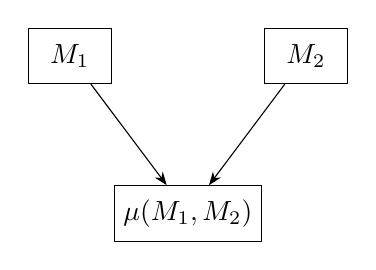
\begin{tikzpicture}[
        box/.style={rectangle, draw, minimum height=2em, minimum width=3em},
        arrow/.style={-Stealth}
    ]
        \node[box] (M1) at (0,0) {$M_1$};
        \node[box] (M2) at (3,0) {$M_2$};
        \node[box] (M) at (1.5,-2) {$\mu(M_1, M_2)$};
        \draw[arrow] (M1) -- (M);
        \draw[arrow] (M2) -- (M);
    \end{tikzpicture}
    \caption{String diagram for merge.}
\end{figure}

\begin{thebibliography}{9}
\bibitem{lawvere2009conceptual}
F. W. Lawvere and S. H. Schanuel, \emph{Conceptual Mathematics}, 2nd ed., Cambridge University Press, 2009.
\bibitem{mac2013categories}
S. Mac Lane, \emph{Categories for the Working Mathematician}, 2nd ed., Springer, 2013.
\bibitem{illusie1971complexe}
L. Illusie, \emph{Complexe Cotangent et D{\'e}formations I}, Springer, 1971.
\bibitem{lurie2009higher}
J. Lurie, \emph{Higher Topos Theory}, Princeton University Press, 2009.
\bibitem{milewski2019category}
B. Milewski, \emph{Category Theory for Programmers}, Blurb, 2019.
\bibitem{hairer2014theory}
M. Hairer, \emph{A Theory of Regularity Structures}, Inventiones Mathematicae, 2014.
\bibitem{daprato2014stochastic}
G. Da Prato and J. Zabczyk, \emph{Stochastic Equations in Infinite Dimensions}, 2nd ed., Cambridge University Press, 2014.
\end{thebibliography}

\end{document}